\documentclass{article}


% if you need to pass options to natbib, use, e.g.:
%     \PassOptionsToPackage{numbers, compress}{natbib}
% before loading neurips_2023

% ready for submission
\usepackage[final]{neurips_2023}

% to avoid loading the natbib package, add option nonatbib:
%    \usepackage[nonatbib]{neurips_2023}


\usepackage[utf8]{inputenc} % allow utf-8 input
\usepackage[T1]{fontenc}    % use 8-bit T1 fonts
\usepackage{hyperref}       % hyperlinks
\usepackage{url}            % simple URL typesetting
\usepackage{booktabs}       % professional-quality tables
\usepackage{amsfonts}       % blackboard math symbols
\usepackage{nicefrac}       % compact symbols for 1/2, etc.
\usepackage{microtype}      % microtypography
\usepackage{xcolor}         % colors
\usepackage{graphicx}       % figures


\title{MLPC Report 2024}


% The \author macro works with any number of authors. There are two commands
% used to separate the names and addresses of multiple authors: \And and \AND.
%
% Using \And between authors leaves it to LaTeX to determine where to break the
% lines. Using \AND forces a line break at that point. So, if LaTeX puts 3 of 4
% authors names on the first line, and the last on the second line, try using
% \AND instead of \And before the third author name.


\author{% 
  Team Park \AND
  Wolfram Laube
  \And
  Hugo von König 
  \And 
  Daniel Hörtenhuber 
}


\begin{document}
\maketitle


\begin{contributions}
  Write here briefly and concisely, who of the authors worked on which tasks / questions / etc. \\ \textcolor{gray}{E.g.: Verena Praher did the entire experimental setup, including the data-split and selection of features and pre-processing. Florian Schmid and Paul Primus trained four different classifiers for the task, and Katharina Hoedt was responsible for the evaluation of the classifiers, generating figures and writing the report.}
\end{contributions}

\section{Data Consistency and Quality}
\subsection{Without listening to all recordings (i.e., by examining feature statistics): Are
there any obvious inconsistencies (wrongly labeled audio snippets, outliers,
etc.) in the data?}
\subsection{Listen to some of the recorded words. Are there notable biases in the data
set? Are the collected samples representative of speech commands that will
be encountered once the application has been deployed?}
\subsection{Listen to some of the sounds labeled as “Other”. Which types of sounds can
you identify? Are they representative of everyday sounds in a household?}
\section{Label Characteristics}
\subsection{Concerning the upcoming task of identifying speech commands in everyday
scenes: How would you group the 20 words and audio snippets labeled as
“Other” in classes and why?}
\subsection{Are the resulting classes unbalanced? If so, how much?}


\section{Feature Characteristics}
\label{sec:headings}

\subsection{How are the pre-computed audio features distributed?}
Mel-scaled energies, MFCCs, Centroid, Bandwidth, and Contrasts follow a normal distribution. These features capture aspects like frequency perception, sound "center of mass", frequency spread, and the difference between peak and valley energies in spectral bands, reflecting the tonal and noise characteristics of the sound.

ZCR, YIN, Spectral Flatness, Spectral Flux, Energy, and Power are audio features that exhibit a right-skewed distribution, indicating variations in sound noisiness, pitch, and loudness. These can be normalized using log transformation or square root transformation.

\begin{figure}
\centering
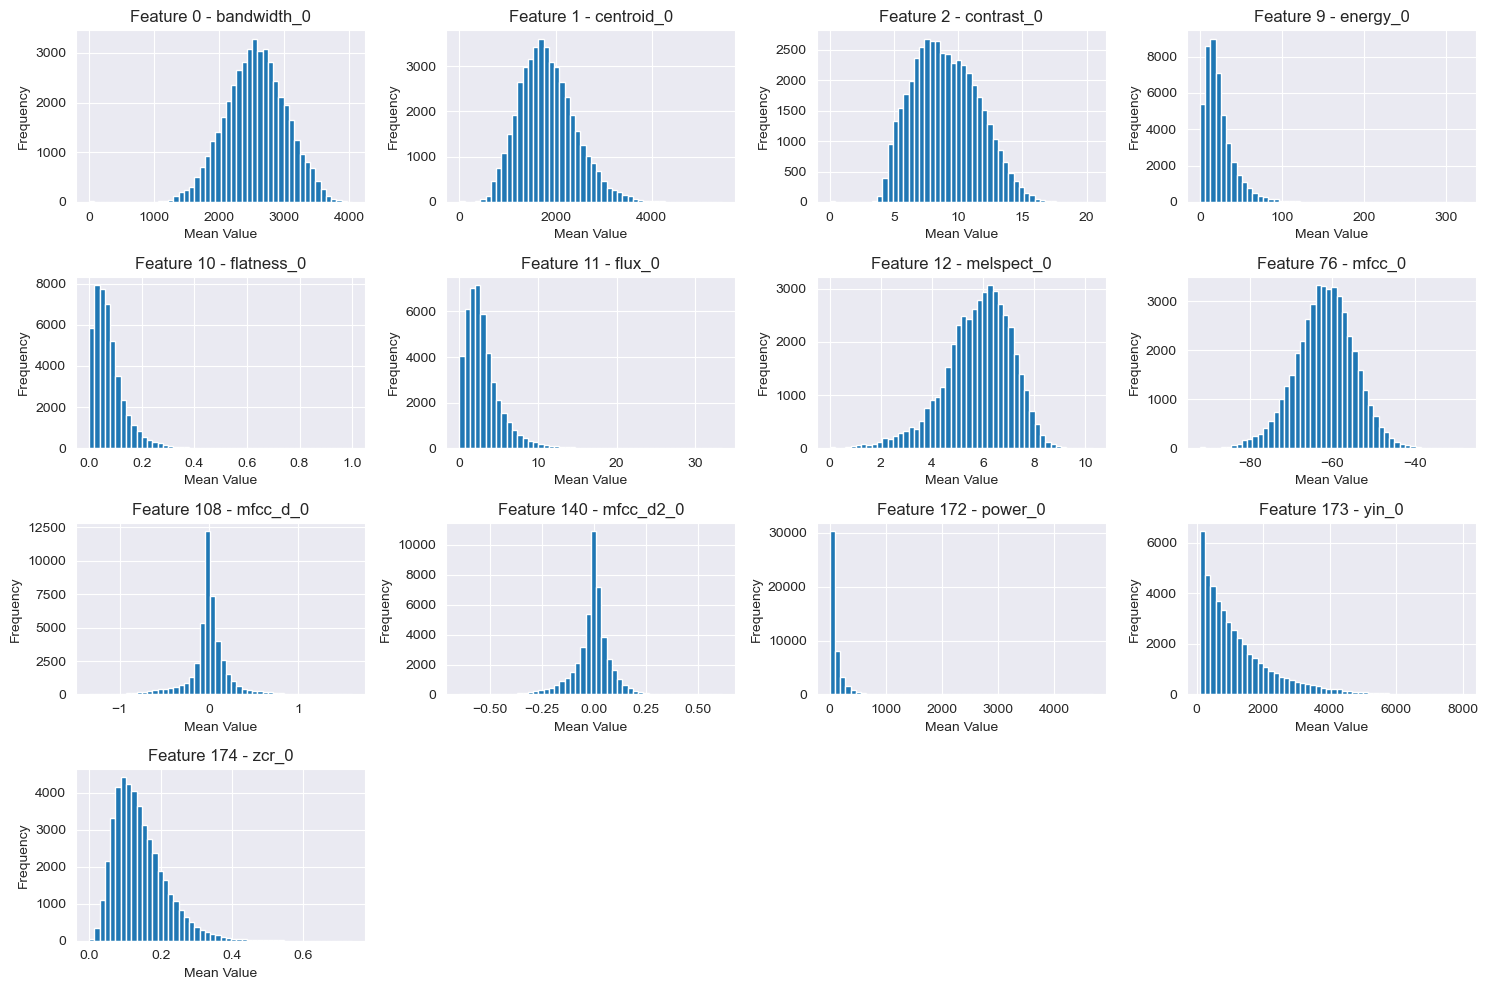
\includegraphics[width=0.8\linewidth]{IMG/3a.png}
\caption{Feature Distribution}
\label{fig:3a}
\end{figure}


\subsection{Are there any pairs or subsets of features that seem highly correlated or
redundant?}
There is a significant correlation between two consecutive mel-scaled energies, that may be seen because similar information is caught in several bins. mel-scaled energies use filter banks across the mel-scale to capture energy, which are overlapping.

Power and energy both exhibit a strong association since they have similar underlying frequency bins. Squaring the energy simply scales the values rather than changing the distribution.

There is also a clear connection between energy and spectral flux, as changes in sound often impact both the spectrum and loudness.

These findings can also be observed from the Correlation Matrix Heatmap.

\begin{figure}[ht]
\centering
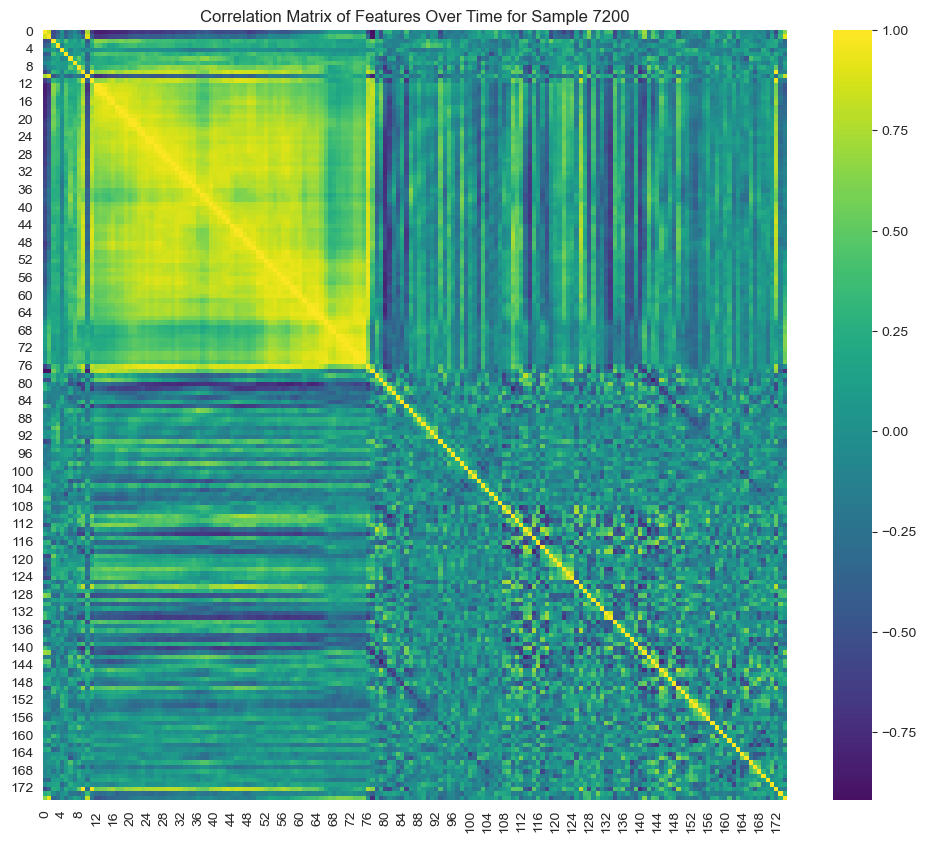
\includegraphics[width=0.4\linewidth]{IMG/3b.png}
\caption{Correlation Matrix Heatmap}
\label{fig:3b}
\end{figure}

\subsection{Are there differences in the feature distributions for different speakers?}
High feature variance between different speakers can have a significant effect on the performance of models due to factors such as accent, pronuncation, tone, and recording quality.

For better performance, speaker normalization can be used, such as Mean and variance normalization, which is a statistical approach that normalizes features to have standard mean and standard deviation, for minimizing the impact of outliers that may be speaker-dependent.

On our Dataset, using Analytics of Variances, we can determine the F-statistics, which can tell us the variation between sample means relative to the variation within the samples. Thus, the higher the value, the greater the evidence that there is a difference between the group means.

The analysis of a random sample of 20 speakers revealed significant differences in feature distribution across speakers. This was evident in the consistently high F-values, ranging from 100 to 550, as well as in the visualization provided by the boxplot.

\begin{figure}[ht]
\centering
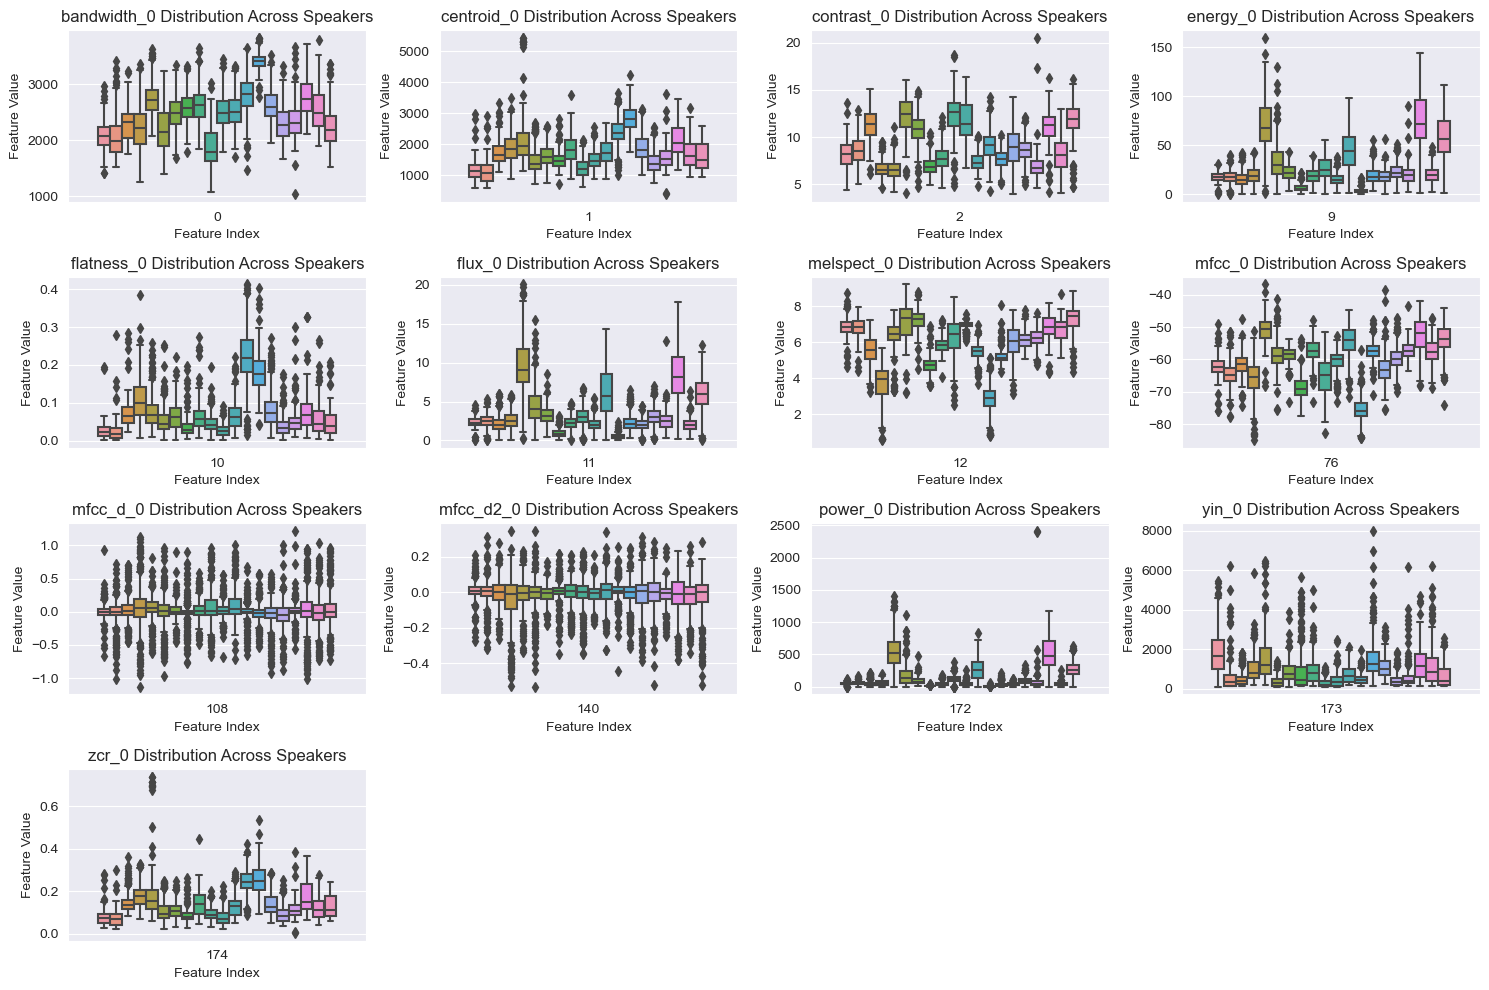
\includegraphics[width=1\linewidth]{IMG/3c.png}
\caption{Feature Distribution for 20 random speakers}
\label{fig:3c}
\end{figure}

\section{Feature / Label Agreement}
\subsection{Which features seem useful for classification? Which ones are correlated with
the labels?}
\subsection{Do similar words (e.g. Haus - aus, Ofen - offen, or nicht - Licht) have a similar
feature distribution?}

\section{Conclusion}
The analysis on Feature Characteristics reveals a variation of distributions and correlations among audio features, pointing to the need for normalization methods to minimize potential biases and enhance model performance.

%%%%%%%%%%%%%%%%%%%%%%%%%%%%%%%%%%%%%%%%%%%%%%%%%%%%%%%%%%%%




\end{document}